% !TeX spellcheck = en_GB

\section{Background}

In order to explore the consequences of adding biological details to a neural system, we need to decide---on a computational and algorithmic level---what task the neural system should ideally perform.
As we mentioned above, we would like to implement eyeblink conditioning by mapping an \LTI system generating a sliding-window transformation (cf.~\Cref{sec:temporal_bases}), specifically, the \LDN system, onto the recurrent Granule-Golgi circuit.
We first provide a review of eyeblink conditioning, followed by an overview of the cerebellar microcircuitry thought to be responsible for this behaviour, and, finally, a discussion of hypothesised mechanisms.

\subsection{Eyeblink conditioning}

\begin{figure}
	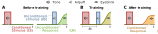
\includegraphics{media/chapters/05_cerebellum/conditioning.pdf}
	\caption[Illustration of eyeblink conditioning.]{
	Illustration of eyeblink conditioning.
	\textbf{(A)} Before training, the animal shows no reaction to the conditioned stimulus (\CS).
	The animal reacts to the unconditioned stimulus (\US), a puff of air into the eye, with an eyeblink.
	\textbf{(B)} During training, both the \CS and the \US are presented with a fixed delay $\Delta t$.
	\textbf{(C)} After training, the animal reacts to the previously neutral conditioned stimulus with an eyeblink. The delay is maintained; the animal begins to close the eye \emph{before} the puff arrives.
	}
	\label{fig:conditioning}
\end{figure}

Eyeblink conditioning is a form of delay conditioning and a widely studied form of motor learning \citep[e.g.,][Chapter~42, pp.~975-979]{kandel2012principles}.
The overall experimental setup is illustrated in \Cref{fig:conditioning}.
Scientists direct a puff of air, the \emph{unconditioned stimulus} (\US), at the eye of an experimental animal.
This triggers the eyeblink reflex, the \emph{unconditioned response} (\UR).
The animal is then repeatedly exposed to the \US paired with a neutral, \emph{conditioned stimulus} (\CS), for example a short tone.
Here, \enquote{neutral} refers to the fact that the animal typically shows no strong reaction to this stimulus.
The \CS precedes the \US by a constant time offset $\Delta t$.

Over time, the subject forms a \emph{conditioned response} (\CR) to the previously neutral \CS, maintaining the fixed delay $\Delta t$. In other words, the subject will learn to have its eye closed $\Delta t$ seconds after the tone, even if the puff is absent.
In our experiments, we use mouse data from \citet{heiney2014cerebellardependent}.
However, this experiment in principle works in most mammals, including humans \citep{cheng2008neural}.
Importantly, the formation of this conditioned response critically depends on the cerebellum.
Ablating the cerebellum causes previously learned \CRpl to be absent \citep{mccormick1981engram}.
This indicates that the cerebellum is not only capable of establishing the connection between the \CS and the \UR, but also of learning the motor trajectory of the response, including the delay.

\subsection{Cerebellar Microcircuitry}
\label{sec:cerebellum_microcircuit}

\begin{figure}[t]
	\centering
	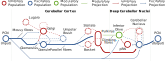
\includegraphics[scale=0.95]{media/chapters/05_cerebellum/cerebellum_anatomy.pdf}
	\caption[Schematic of the cerebellar microcircuit.]{Schematic of the cerebellar microcircuit. Dashed projections and populations are not included in our model. Cerebellar nucleus afferents affect both the excitatory and inhibitory sub-populations.  The main feed-forward pathway is highlighted in bold. \emph{\PCN}~$\hat=$~pre-cerebellar nuclei. \emph{pRN}~$\hat=$~parvicellular Red Nucleus. Data from \citet{ito2010cerebellar,llinas2010olivocerebellar}.}
	\vspace*{-0.5em}
	\label{fig:cerebellum_anatomy}
\end{figure}

Before we continue to discuss the two prevalent theories on how the cerebellum could learn the conditioned response, it is worthwhile to review the cerebellar microcircuitry depicted in \Cref{fig:cerebellum_anatomy}.
Afferent nerves from pre-cerebellar nuclei (\PCN; brainstem and cerebral cortex carrying sensory signals) project as \enquote{mossy fibres} onto granule cells in the cerebellar cortex.
Cerebellar granule cells are tiny and account for the majority of neurons in the mammalian brain.
Thus, small numbers of pre-cerebellar neurons connect onto many granule cells.

Granule cells also have interneurons interspersed amongst them, the Golgi cells.
These form an inhibitory feedback loop with the granule cells.
That is, granule cells excite Golgi cells, and Golgi cells inhibit granule cells \citep{ito2010cerebellar}.
Notably, the connections from Golgi and \PCN to granule cells are formed through so-called glomeruli.
Each granule cell extends to on average four glomeruli and, at each glomerulus, receives input from one pre-cerebellar neuron through a mossy fibre terminal, as well as one or more Golgi cells \citep{palkovits1972quantitative,jakab1988quantitative,chadderton2004integration}.
Furthermore, the connectivity between Golgi and granule cells is spatially constrained.
Golgi cells only connect to granule cells within a \SI{600}{\micro\metre} diameter \citep{albus1971theory,dangelo2013cerebellar}.
The ratio of granule to Golgi cells is about $400$:$1$ \citep{korbo1993total}.

Granule cell axons, the so called \enquote{parallel fibres}, project onto the Purkinje cells, which inhibit neurons in the cerebellar nucleus, and in turn project back onto the brainstem and cerebral cortex \citep{ito2010cerebellar,llinas2010olivocerebellar}.
So-called \enquote{climbing fibres} project from Inferior Olive neurons in the deep cerebellar nucleus onto Purkinje cells. 
Evidence suggests that activity in the climbing fibres is responsible for modulating the synaptic strength of granule to Purkinje projections.
Climbing fibre activity is often interpreted as an \enquote{error signal} $\epsilon(t)$ responsible for driving learning in the cerebellar cortex \citep{ito2010cerebellar}.

\subsection{Hypothesised Mechanisms Supporting Delay Learning}

There is no current consensus on what the exact mechanism is that supports delay learning in the cerebellum.
Specifically, there are two competing hypotheses: the classic adaptive filter theory and the view that intrinsic properties of the Purkinje are responsible for timing.
%We review these ideas in more detail below.

\subsubsection{Adaptive filter hypothesis}
As originally pointed out by \citet{marr1969theory,albus1971theory}, the massive divergence (number of post-neurons for a single pre-neuron) and small convergence (number of pre-neurons for a single post-neuron) in the \PCN to granule projection suggests that granular cells are tuned to specific patterns of activity in the \PCN.
Modulating the synaptic weights between the granule and the Purkinje cells using the climbing fibre error signal can be used to recombine the sparse pattern detectors and to decode arbitrary functions.

The adaptive filter hypothesis, originally proposed by \citet{fujita1982adaptive}, can be interpreted as extending this idea toward temporal tuning.
That is, similarly to what we discussed in the previous chapter,
granule cell activity does not only depend on the current \PCN activities, but on their past history.
Correspondingly, if this temporal tuning is diverse enough, that is, granule cells are sensitive to different time-courses, this will form a suitable temporal basis from which functions over time, such as delays, can be decoded.
A possible source for the temporal tuning could be the recurrent granule-to-granule connections that are mediated by the inhibitory Golgi cells.
Indeed, \citet{rossert2015edge} find that randomly connecting the Golgi and granule cells generates diverse tuning that can be exploited as a temporal basis.
Our contribution is to test whether optimal temporal tuning---i.e., an \LTI system approximating a sliding-window transformation (cf.~\Cref{sec:temporal_bases})---could be realised in the Granule-Golgi circuit.


\subsubsection{Intrinsic properties of the Purkinje cells}
A more recent theory is that responses observed in tasks such as eyeblink conditioning inherently rely on intrinsic properties of the Purkinje cells.
In other words, the Purkinje cells act as \enquote{time cells} \citep{lusk2016cerebellar}, and the temporal properties of the granule cells play a lesser role.
Instead, climbing fibre input triggers processes within the Purkinje cell and their dendritic structures that are responsible for the formation of a delayed output.
Evidence for this comes from \citet{johansson2014memory}, who find that bypassing the granule cells and directly injecting signals into the parallel fibres still evokes a previously learned delayed response from the cerebellum, albeit a weaker one.


\subsubsection{Discussion}
We think that these two theories are not inherently contradictory.
Both temporal tuning of the granular cells and intrinsic temporal properties of the Purkinje cells could play a role in delay learning---as we discussed in \Cref{chp:temporal_tuning}, both the intrinsic dynamics of neurons, and the network dynamics can in principle be harnessed to produce desired dynamics.

The findings in this chapter provide a strong argument that the Granule-Golgi circuit is well-suited for implementing some kind of temporal basis, and as such confirms the results of previous studies \citep[cf.][]{dean2010cerebellar,rossert2015edge}.
Still, our work only takes a fraction of the available data on cerebellar neurophysiology into account and as such should not be seen as strong evidence for or against either of the two proposed mechanisms.
